\documentclass[a4j,12pt,landscape]{jarticle}
\topmargin=3mm \headheight=0mm \headsep=0mm
\textheight=170mm 
\textwidth=220mm
\evensidemargin=0mm \oddsidemargin=0mm
\footskip=0mm
\parindent=0cm

%\usepackage[all]{xy}
\usepackage{amssymb}
\usepackage{amscd}
\usepackage{amsmath}
\usepackage{graphics}
\usepackage{graphicx}
\usepackage{amsthm}

\pagestyle{empty}

\def\modulo{{\rm mod}}
\def\F2{{\mathbb F}_2}
\def\wt{{\rm wt}}
\def\wo{{\rm wt}_o}
\def\wf{{\rm wt}_f}
\def\UL{{\rm ul}}
\def\bx{{{\mathbf x}}}
\def\by{{{\mathbf y}}}
\def\bw{{{\mathbf w}}}
\def\bu{{{\mathbf u}}}
\newcommand{\lshift}[1]{{\large $\mbox{#1}\atop<<$}}
\newcommand{\rshift}[1]{{\large $\mbox{#1}\atop >>$}}

\title{}
\author{}
\date{\today}

\begin{document}
\Huge

\vspace*{2cm}
\begin{center}
{\bf Simple and Fast MT:\\
  A Two times faster new variant of \\
  Mersenne Twister}
\vspace{1cm}

Mutsuo Saito (Hiroshima Univ.) \\
and \\
Makoto Matsumoto (Hiroshima Univ.).
\end{center}
\vspace{\fill}
This research is granted by 
\newpage

\newpage
\noindent
{\bf 1. Pseudo Random Number Genarator}\\

In this talk, PRNG is a (finite state) automaton consisting of:
\begin{itemize}
\item State set $S$. 
\item Transition function $f:S \to S$.
\item Initial state $s_0 \in S$.
\item (No imput considered.)
\end{itemize}
Change the state as follows:
$$
s_0 \mapsto s_1:= f(s_0) \mapsto s_2:=f(s_1) \mapsto \cdots.
$$

\newpage
Let $O$ be the set of output symbols.

(In this talk, we assume $O$=32-bit integers.)

\vskip 1cm
At each state $s$, 
the output is determined by 
\begin{itemize}
\item an output function $o:S \to O$.
\end{itemize}
The output sequence becomes
$$
o(s_0),o(s_1),o(s_2),\ldots.
$$
We use this as a pseudo-random sequence.
\newpage
\begin{center}
\includegraphics[width=0.7\linewidth]{figure01.eps}
\\
Figure 1: Automaton.
\end{center}

 
\newpage
\noindent
{\bf 2. Feedbacked Shift Regiter}\\
In the above automaton, 
its period is bounded  \\
by the number of the states $\#(S)$.

\vskip 5mm
We want large $S$ (like 20000 bits), \\
which admits fast computation of $f$ \\
in a software implementation.

\vskip 5mm
Feedbacked Shift Register (FSR) permits $f$ \\
with $O(1)$-time complexity.

\newpage
Feedbacked Shift Register.
\begin{itemize}
\item
$S=$an array of words(=32-bit integers) of length $N$:
$$
S = \{(\bw_0,\ldots,\bw_{N-1})| \bw_i \mbox{: 32-bit integer}\}.
$$
\item
$f:(\bw_0,\ldots,\bw_{N-1}) \mapsto (\bw_1,\ldots,\bw_{N-1}, \by)$,

where $\by$ is given by a function $g$
$$\by:=g(\bw_0,\ldots,\bw_{N-1}).$$
\end{itemize}

Round robin reduces the computation of $f$ to that of $g$. 

For high speed generation, $g$ looks at only a few words \\
in the state array.
\newpage

\begin{center}
\includegraphics[width=0.7\linewidth]{figure02.eps}
\\
Figure 2: Feedbacked Shift Register.
\\
\end{center}
\newpage
\noindent
{\bf 3 Linear Generator}

We identify: 
\begin{itemize}
\item 
a bit $\{0,1\}$ with the two element field $\F2$, and
\item 
32-bit integer with horizontal vector $\F2^{32}$.
%\item 
%128-bit integer with horizontal vector $\F2^{128}$.
\item 
Regard $S$ as an $\F2$-vector space.
\end{itemize}
An automaton is said to be {\em $\F2$-linear} if 
the transition function $f$ and 
the output function $o$ are both $\F2$-linear. \\
~~~We consider only this kind of automata, with 
justification:
\begin{itemize}
\item the period is computable
\item some kinds of assurance on the distribution \\
(such as the dimension of equidistribution) can be given
\item can be converted to a non-linear sequence 
by using a non-linear transform. 
\end{itemize}

\newpage
\noindent
{\bf 4. Examples of Linear FSR}

{\bf GFSR} ('73, Lewis-Payne)
$$
g(\bw_0,\ldots,\bw_{N-1}) = g(\bw_0, \bw_M) = \bw_0 + \bw_M.
$$
The function $g$ reads only two words, so this is called \\
a two-tap FSR.

Period is $2^N-1$.

\newpage
{\bf Twisted GFSR} ('92, '94, Matsumoto-Kurita)
$$
g(\bw_0,\ldots,\bw_{N-1}) = g(\bw_0, \bw_M) = \bw_0A + \bw_M,
$$
where $A$ is a ($32\times 32$)-matrix over $\F2$, defined by
$$
\bx A = 
\left\{\begin{array}{ll}
  \mbox{shiftright}({\bf x}) & (\mbox{if LSB of $\bx$ is 0}) \\
  \mbox{shiftright}({\bf x})\oplus{\bf a} & 
  (\mbox{if LSB of $\bx$ is 1}),
\end{array}\right.
$$
where ${\bf a}$ is a constant vector.
Period is $2^{32N}-1$. 
\begin{center}
\includegraphics[width=0.6\linewidth]{figure03.eps}
\\
Figure 3: Twisted GFSR
\end{center}
\newpage
{\bf Mersenne Twister} ('98 Matsumoto-Nishimura)
$$
g(\bw_0,\ldots,\bw_{N-1}) = g(\bw_0, \bw_1, \bw_M) = (\bw_0|\bw_1)A + \bw_M,
$$
where $(\bw_0|\bw_1)$ denotes
the concatenation of $32-r$ MSBs of $\bw_0$ and $r$ LSBs of $\bw_1$,
and $A$ is the same as above.

Period is $2^{32N-r}-1$, chosen to be a Mersenne prime.

\newpage
\noindent
{\bf 6 Speed Up PRNG}

{\bf 6-1} Speed Up transition function

The speed of PRNG mainly depends on
the speed of transition function.\\
~~~~Recent CPU archetecture has SIMD (Single Instruction Multiple
Data) instruction set with 128-bit SIMD registers.

The recursion formula is
\[x_{n+i} = Ax_{n-1+i} + Bx_{n-2+i}+ Cx_{m+i} + Dx_{i},\]
where each of $x_i$ is a 128-dimensional vector over the two 
element field ${\mathbb F}_2$ and
$A$, $B$ and $C$ are $128 \times 128$ matrices over
${\mathbb F}_2$.

\begin{center}
\includegraphics[width=0.7\linewidth]{simd-shift.eps}
\\
Figure 5: Sample of SIMD instructon.
\end{center}
%Some people implement MT19937ar using SIMD instruction set.
%It fast. But we think it's much faster when the recursion formula is
%designed to fit for SIMD instruction set.
\newpage
Endian\\
When use 32-bit and 128-bit integers together,

\begin{center}
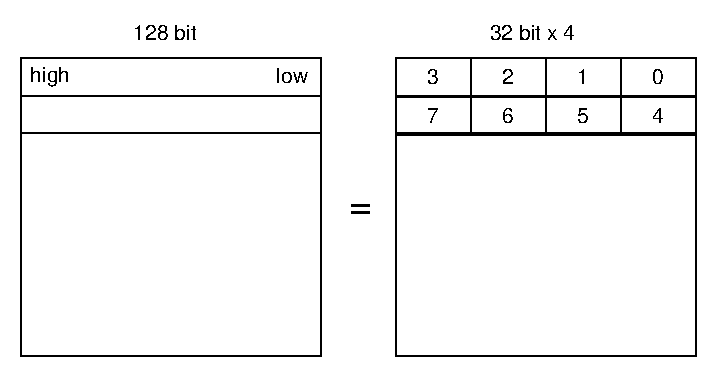
\includegraphics[width=0.7\linewidth]{little-endian.eps}
\\
Figure 5: Little Endian
\end{center}
\newpage
{\bf 6-2} Speed Up of output function

MT19937ar calculates next 624 states at once,
and output pseudo-random numbers sequencially.

\vspace{\baselineskip}
if (mti $>$= N) \{\\
~~~~calculate next 624 states.\\
\}\\
tempering...\\
output.\\

The condition part of {\bf if} statement is evaluated every time.
And jump instruction may be executed every time.

We think it's much faster when PRNG outputs
some blocks of numbers at once.

\newpage
Here is the rough scketch of {\bf fill\_array\_block} function.

The idea of {\bf fill\_array\_block}
\begin{center}
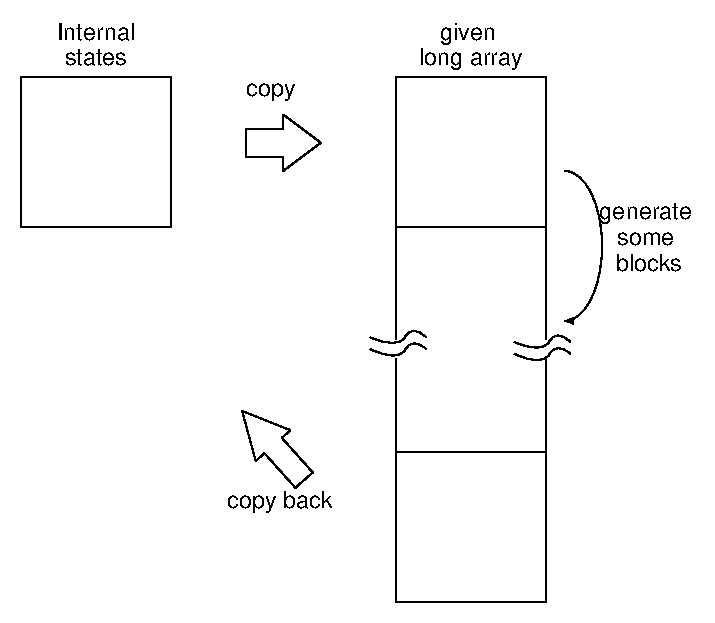
\includegraphics[width=0.7\linewidth,height=0.7\textheight,
keepaspectratio]{fill_array.eps}
\\
Figure 6: fill\_array
\end{center}
\newpage
And Figure 6 is same as following steps.


Step 1. (first N - M words) \\
~~~~Read from the internal memory and write to the given array.

Step 2. (N - M + 1 to N words) \\
~~~~Read from the internal memory and given array, and 
write to the given array.

Step 3. (some multiple of 624 words + 624 - M words)\\
~~~~Read from the given array and write to the given array.

Step 4. (last N words)\\
~~~~Read from the given array and write to the given array and
 the internal memory.

Step 5. (MT only)\\
~~~~Temper the all elements of given array. 
\newpage
\noindent
{\bf 7 Simple and Fast MT (SFMT)}

Now one word is 128-bit width,
and we read $\bw_{N-1}$ and $\bw_{N-2}$.

\begin{center}
%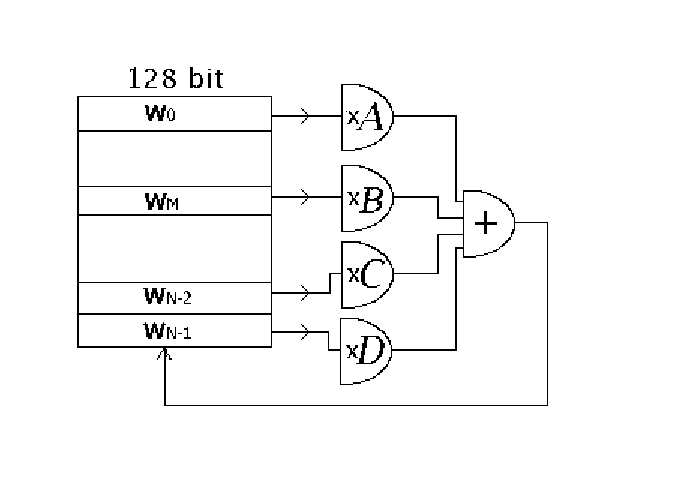
\includegraphics[width=0.7\linewidth]{sfmt-a.eps}
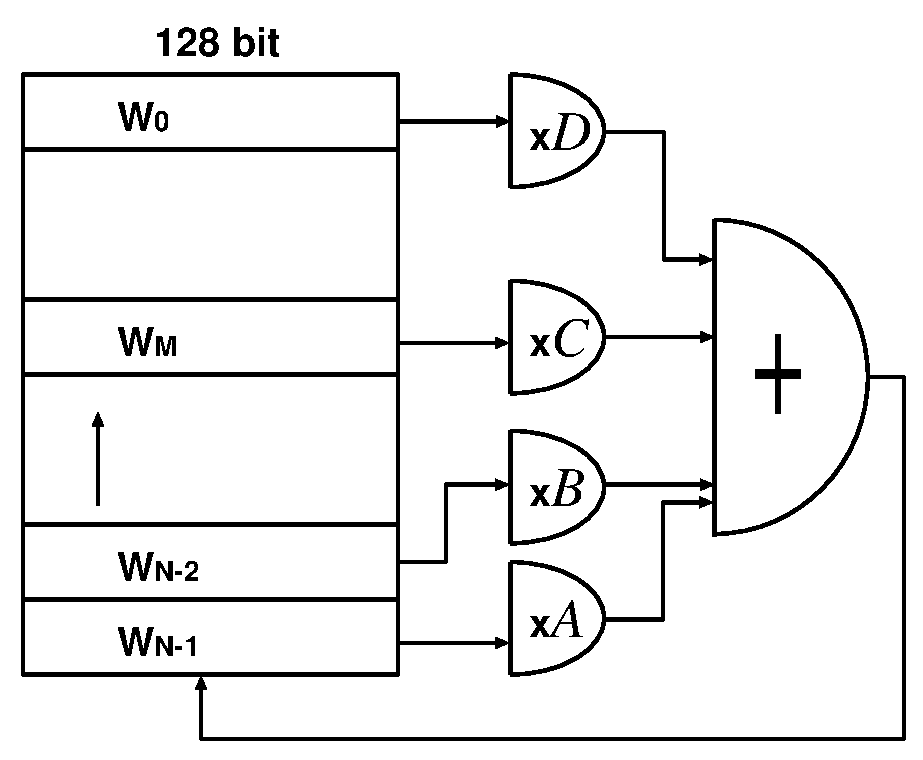
\includegraphics[width=0.7\linewidth]{sfmt-a2.eps}
\\
Figure 6: The transition function of Simple and Fast MT
\end{center}
SFMT is currently implemented for Intel's SSE2 and PowerPC's altivec SIMD
instruction set.


\newpage
Figure 8 shows an implementation SFMT19937 with period
$2^{19937}-1$.  The function \lshift{128} $n$ is left shift $n$ bit
regarding the word as 128 bit integer, and the function \lshift{32} $n$ is
lesft shift $n$ bit regarding the word as four 32-bit integers
(\rshift{128} and \rshift{32} are shift right).

\begin{center}
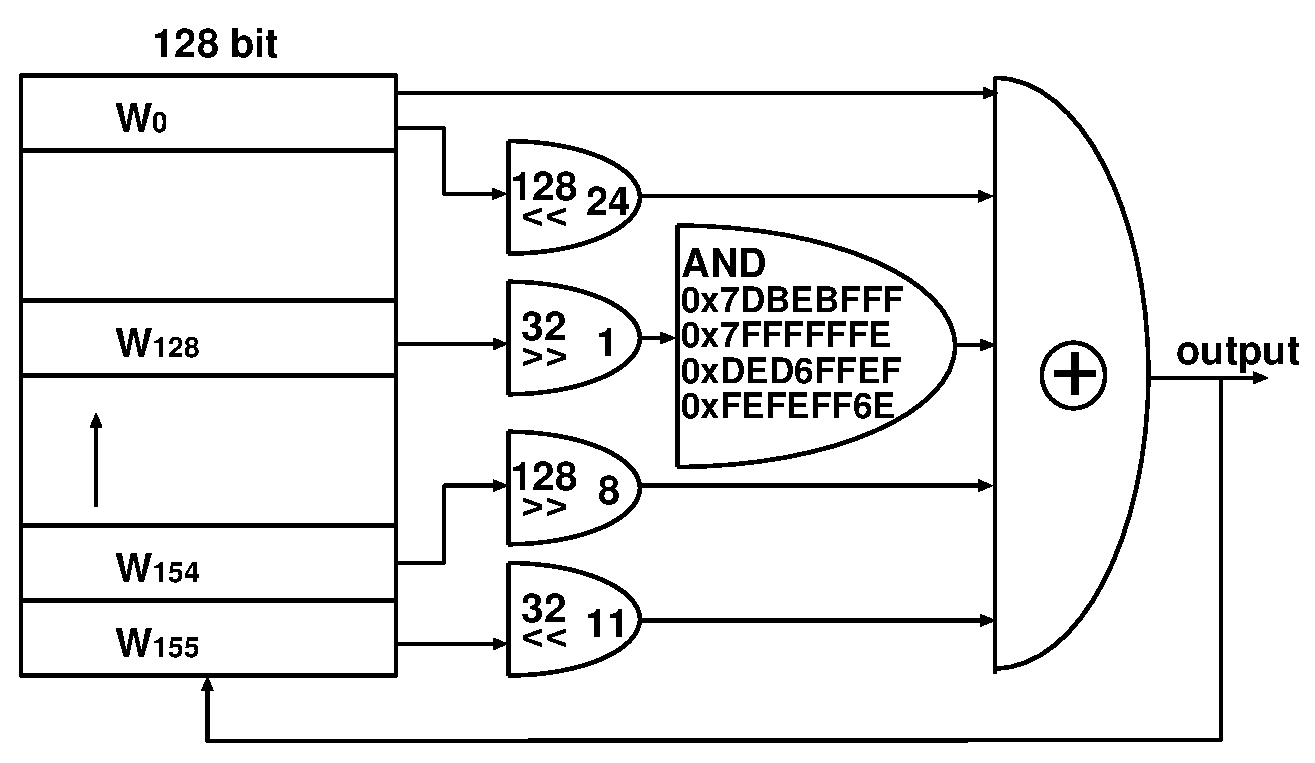
\includegraphics[width=0.7\linewidth]{sfmt-b2.eps}
\\
Figure 8: Detailed description of SFMT19937.
\end{center}

\newpage
{\bf 7-1} Initial Value\\
The internal state S of SFMT is decomposed to:
$$
S = S_{19937} \oplus S_{31}
$$

If start with some special internal status,
it may occur that $S_{19937}$ is zero.
And the period of PRN becoms less than $2^{31}-1$.

To avoid this special internal status and to assure
the period greater than $2^{19937}-1$,
we set the special 32-bit value (initila value) in 
initial internal state.

The initial value for SFMT19937 of Figure 8 is 0x4d734d6d.
This value is set to the heighest 32-bit of the first 128-bit
word.

\newpage
{\bf 7-2} The period of 32-bit output.\\
SFMT has the period of least $2^{19937}-1$ as 128-bit output PRNG.
Every 128-bit output can be used four 32-bit output, then
SFMT has the period at least $2^{19937+4}-1$ as 32-bit output PRNG.

The reason of additional length of the period is additional 
internal state by the counter which indecates the position of
the output 32-bit in the 128-bit. 

\newpage
\noindent
{\bf 7-2} High dimensional distribution.

{\bf Definition.} 
A periodic sequence with period $P$
$$\bx_0, \bx_1, \ldots, \bx_{P-1}, \bx_P=\bx_0, \ldots$$
of $v$-bit integers is said to be {\em $k$-dimensionally equidistributed}
if any $kv$-bit pattern occurs equally often as a $k$-tuple
$$
(\bx_i, \bx_{i+1}, \ldots, \bx_{i+k-1})
$$
for a period $i=0,\ldots, P-1$. 

(The all-zero pattern occurs once less often.)

\newpage
A periodic sequence of 32-bit integers is said to be
{\em $k$-dimensionally equidistributed with $v$-bit accuracy}
if the most significant $v$ bits of each integer are
$k$-dimensionally equidistributed. 

We denote by $k(v)$ the maximum such $k$. 

\vskip 5mm
We have an upperbound 
$$
k(v) \leq \lfloor \log_2 (P+1) / v \rfloor, 
$$
and define the dimension defect as the summation of the gaps 
$$
\Delta_1 := \sum_{v=1}^{32}(\lfloor \log_2 (P+1) / v \rfloor -k(v)).
$$

\newpage
{\bf 7-3} Calculate 32-bit $k(v)$ of 128-bit recursion formula PRMG

\begin{center}
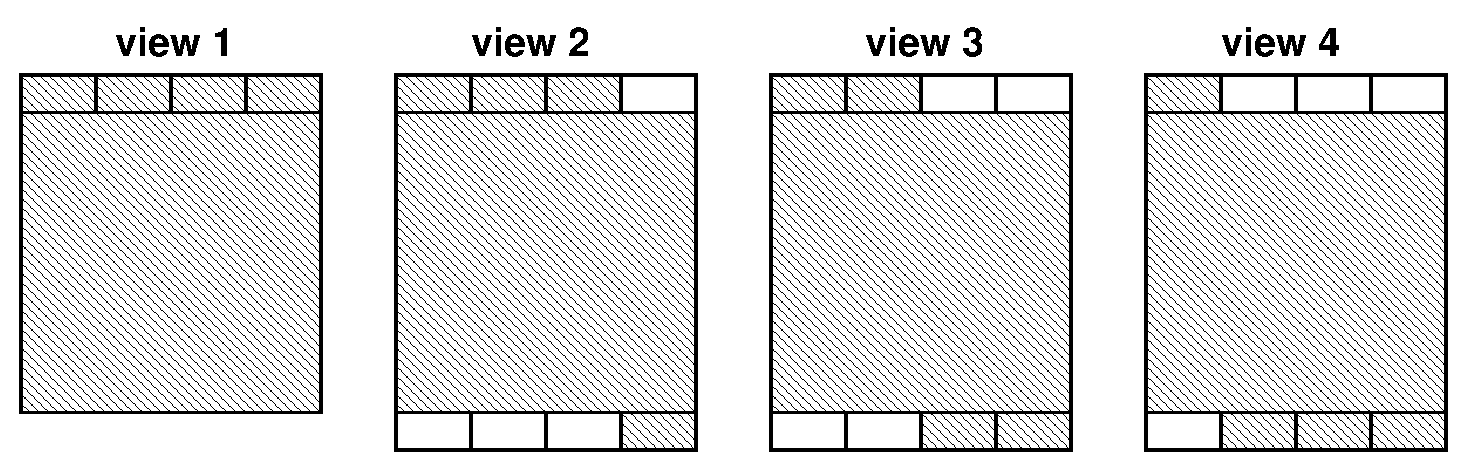
\includegraphics[width=\linewidth,height=0.6\textheight,
keepaspectratio]{view.eps}
\\
Figure 9: get minimum $k$-distributio of four views
\end{center}
\newpage

\begin{center}
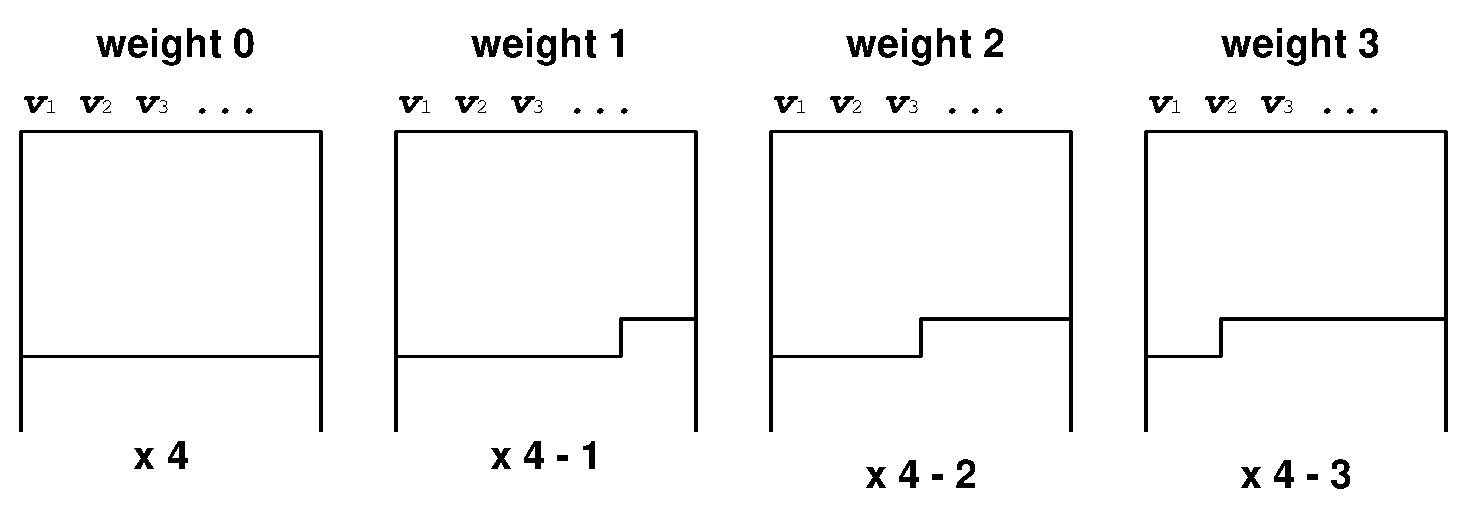
\includegraphics[width=\linewidth,height=0.6\textheight,
keepaspectratio]{weight.eps}
\\
Figure 9: weighted norm
\end{center}

\newpage
{\bf 8 Comparison of Randomness}
\begin{center}
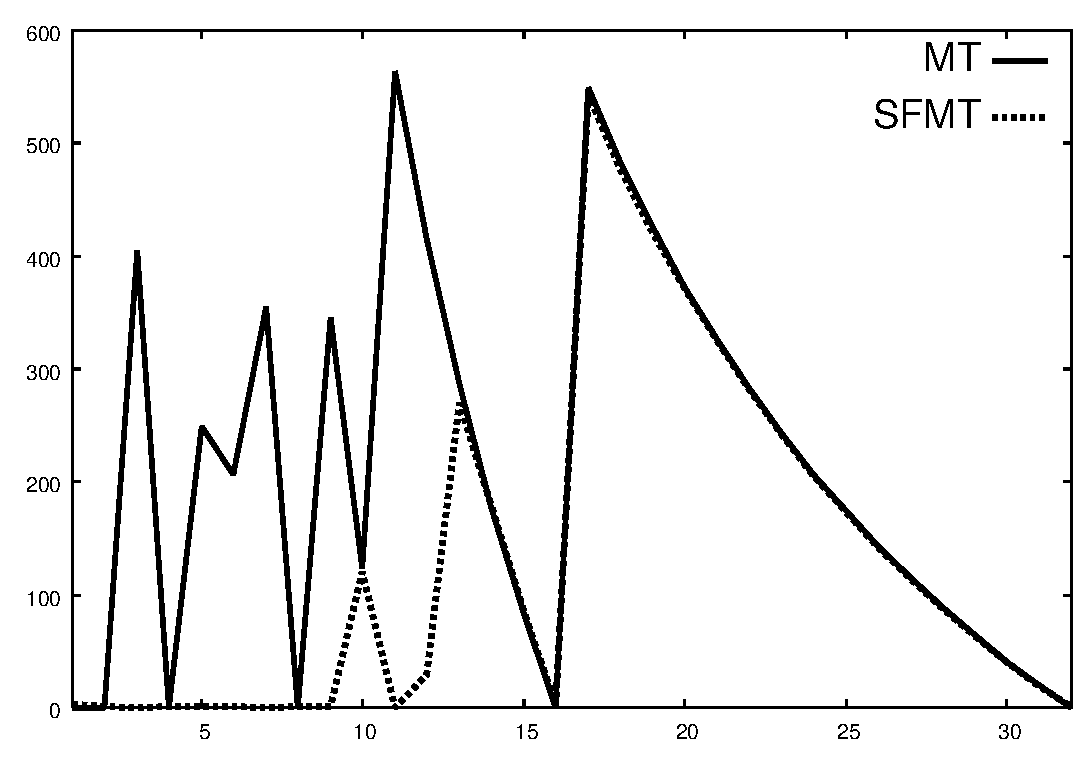
\includegraphics[width=0.7\linewidth,height=0.6\textheight,
keepaspectratio]{delta.eps}
\\
Figure 9: gaps form upperbound
\end{center}
\begin{center}
\LARGE
\begin{tabular}{crr} \hline
  & MT19937 & SFMT19937 \\ \hline\hline
  $\Delta_1$ & 6750 & 5089 \\
  $k(1)$ & 19937 & 19931 \\
  $k(32)$ & 623 & 622 \\ \hline
\end{tabular}
\end{center}
\newpage
\noindent
{\bf 9 Comparison of speed}
\begin{description}
  \item Generators
    \begin{itemize}
    \item MT19937: Mersenne Twister with period $2^{19937}-1$ ('98).
    \item MT(SIMD): MT19937 using SIMD instruction set.
    \item SFMT19937: Simple and Fast MT with period $2^{19937}-1$.
    \item SFMT(SIMD): SFMT19937 using SIMD instruction set.
    \end{itemize}
  \item CPUs
    \begin{itemize}
    \item Intel Pentium M 1.4GHz
    \item AMD Athlon64 
    \item Freescale Power PC 1.33GHz
    \end{itemize}
  \item Output functions
    \begin{itemize}
    \item fill\_array\_block output
    \item sequencial output (old normal style)
    \end{itemize}
  \end{description}

\newpage
\begin{center}
\begin{tabular}{|c|c||c|c|c|c|c|}
\hline
CPU & output & MT & MT{\Large(SIMD)} & SFMT & SFMT{\Large (SIMD)} & {\Large compiler} \\
\hline \hline
{\Large Pentium M}  & block & 0.903 & 0.479 & 0.584 & 0.256 & gcc\\ \cline{2-6}
{\Large 1.4GHz} & seq & 1.112 & 1.016 & 1.007 & 0.776 & \\ \hline
{\Large Pentium IV} & block & 0.498 & 0.300 & 0.387 & 0.175 & intel\\ \cline{2-6}
{\Large 3GHz} & seq & 0.847 & 0.724 & 0.648 & 0.449 & \\ \hline
{\Large Athlon} & block & 0.543 & 0.264 & 0.272 & 0.112 & intel \\ \cline{2-6}
{\Large 3800+} & seq & 0.487 & 0.319 & 0.407 & 0.312 & \\ \hline
{\Large Power PC G4}  & block & 1.406 & 0.479 & 0.919 & 0.176 & gcc\\ \cline{2-6}
{\Large 1.33GHz} & seq & 0.942 & 0.543 & 0.974 & 0.495 &\\ \hline
\end{tabular}
\\
\vskip 5mm
\begin{tabular}{|c|c|} \hline
  block & 616 calls of 128 blocks fill\_array\_block \\ \hline
  seq & 624 $\times$ 128 $\times$ 616 = 99999744 calls\\ \hline
\end{tabular}
\\
\vskip 5mm
Table 1. Comparison of the time (sec.) to generate $10^8$ prns.
\end{center}
\newpage
\noindent
{\bf 9 Concluding Remarks}
\begin{itemize}
\item We proposed Simple and Fast Mersenne Twister (SFMT). 
\item Almost two times faster than Mersenne Twister.
\item Better $k(v)$ than MT19937 \\
(totally better, but in some point worse than MT).
\end{itemize}
We conclude that SFMT is fast version of Mersenne Twister.

\end{document}




